\chapter{The informatics of biology}
Bioinformatics is the application of computational methods to biological problems,
either by analysing large amounts of data or by replacing experiments with computer programs.

\section{Predictors}
A significant fraction of the protein bioinformatics work is the development of predictors: statistical or machine learning methods that can, given limited information, predict properties of proteins.
A common choice is to make predictions taking only the amino acid sequence, because this is the easiest information we can acquire of a protein.
Other methods may require extra annotation, such as Gene Ontology -- an annotation condensing all our knowledge of the gene that produced the protein -- or 3D structures -- experimental or models.

\section[Multiple Sequence Alignments]{Increasing statistics: Multiple Sequence Alignments}
Proteins, as organisms, are products of evolution, so we can find similar versions of the same protein in different organisms.
Even when the function is novel, it usually evolves as a minor modification on pre-existing proteins.
This means that, in most cases, we can obtain a better prediction when working at the \emph{family level,}
i.e., considering not only our protein of interest, but also any related sequence in our database.

In order to have coherent statistics, every sequence must be aligned to the original query, as in the following example:

\begin{center}
\marginpar{\phantom{a}}
\marginpar{\phantom{a}}
\marginpar{\phantom{a}}
\marginpar{An example MSA}
\begin{Verbatim}[fontsize=\small, xleftmargin=1em]
1       10        20        30        40        50   
FCLEPPYTGPCKARMIRYFYNARSGSCETFIYGGCKAKRNNFKSEEDCMRTCG
FCREPPYTGPCSAHFVRYFYNATTGLCQSFVYGGCRGKQNNFMDEKECLHTCD
FCREPPYTGPCRAHFIRYFYNATTGLCQTFVYGGCRGKQNNFMDEKECLHTCD
ICSMKNDTGPCKAYMPRWFFNSQTKQCEEFIYGGCSGNNNNFMTREDCCNSCS
-CTLPKVPGPCNAYFVRWWYDQQKEICSSFIYGGCQGNNNNFQSESVC-----
------DPGPCKAYMPRFYFEIEKKECQEFIYGGCGGNENRFFTKRECQRICK
ECLMAPDPGNCGGVRERWFFSPEAKQCRLFGYSGCQGNANNFATIEDCMAKC-
LCHLAMESGPCRAAKPRWYFDQGKQTCVEYIYGGCRGNSNNFETKAECMRTCS
-CEQAMDPGPCKAAFPRWYFNSQTGQCEQFIYGGCLGNDNNFVTEQECQTTCG
\end{Verbatim}
\end{center}

The collection of sequences is called a Multiple Sequence Alignment, or MSA, and the dash \texttt{-} indicates a gap, a residue that is not present at that particular position.
This section explains how to build it.


\subsection{Pairwise alignment}
The building block of an MSA is the alignment of each related sequence to our query, and the first step is measure how similar they are.
The most basic scheme is simply count the number of matching amino acids, assigning a positive score for matches, and a penalty for mismatches.

Proteins \marginpar{The reason for gaps} have insertions and deletions, which means the matching regions in different proteins may be discontinuous.
We can allow for gaps in the scores including a term that considers both opening -- our belief of how common insertions and deletions are -- and extending the gap -- considering our expectation of their length.

Furthermore, not all mismatches are the same.
For example leucine (L) and isoleucine (I) are functionally very similar, and can often be replaced without loss of function.
On the other hand, a single mutation from glutamic acid (E) to valine (V), in humans is enough to cause sickle cell anaemia.

Nor are all matches.
Alanine (A) forms over $7\%$ of the proteome, so we are more likely to find a hit at random than with tryptophan (W), which forms less than $2\%$.

We can codify \marginpar{Substitution matrix} the difference between different amino acids in a substitution matrix.
The most common choice to detect distant related proteins is the \texttt{BLOSUM} family.
\citet{blosum} derived them from a set of 500 multiple sequence alignments.

\subsection{Scaling up: BLAST}
Performing a pairwise alignment on a large sequence database would be very slow, but for a given query, most entries in the database are not related.
Programs like BLAST (Basic Local Alignment Search Tool) introduce a set of heuristics to discard negatives as quickly as possible.
They do not guarantee an optimal alignment according to the scoring matrix, but this is offset by a much higher amount of data.

\subsection[PSSMs and PSI-BLAST]{Position Specific Scoring Matrices and PSI-BLAST}

Substitution matrices assume a fixed evolution model, and that every residue is as important as every other.
But this is not true, we can observe that some protein regions are highly conserved because they are, in one way or another, important for the function of the protein.
In the earlier example, we can see how around column 40, there are fewer changes.
We want our search to reflect this fact, and, for instance only accept changes in these regions if they provide enough similarity in the rest of the protein to support the fact that they are related.

PSI-BLAST does this using an iterated search, and building Position Specific Scoring Matrices (PSSM).
The first iteration is a normal BLAST search, using the default substitution matrix, but in the subsequent iterations, it uses the statistics of each column to update the substitution matrix.
Since each position is treated independently, it can model better the importance of each residue.

\subsection[Hidden Markov Models]{Increasing sensitivity with Hidden Markov Models}
PSSMs can model the differences in probabilities for each amino acid at different positions, but gaps are still modelled with a flat penalty across the sequence.
We know this is not a good representation of proteins, since they are unlikely to happen in the core, due to the lack of space.
Insertions are easy to introduce in short, external loops; and deletions are most likely in long loops. 
A representation that allows us to model both mutations and insertions and deletions with different rates at different positions are Hidden Markov Models (HMM).

An HMM \marginpar{The HMM} is a probabilistic model, where the system travels across a series of hidden states following a Markov chain, a model with discrete states where the probability of transition depends only on the current state -- ignoring the history.
We do not have access to these states -- hence \emph{hidden}.
Instead, each of them has a certain probability of emitting a symbol: the observed amino acids.
Fitting a Hidden Markov Model consists on figuring the emission probability for each state -- the analogue to the PSSMs -- and the transition probability between states.
Like in PSI-BLAST, this is done iteratively, passing several times through the data and updating our belief.

The two most popular programs to perform this searches are JackHMMER \citep{jh}, and HHBlits \citep{hhblits}:

\begin{itemize}
\item JackHMMER compares every sequence in the database with its HMM.
It performs a HMM-sequence comparison.
\item HHBlits uses a database of pre-computed HMMs based on sequence clusters.
It compares HMM to HMM, and in case of a match, includes all the members of the cluster in the MSA.
\end{itemize}

JackHMMER is slower, 
\marginpar{Advantages and disadvantages}
because it must consider each sequence; but it can search against any database without the need to pre-prepare it.
JackHMMER can easily keep an up-to-date sequence database, or work on databases tailored for the search at hand.

On the other hand, each HHBlits search is faster since it only needs to compare once against each cluster, but it requires a lot of computational resources to perform the initial clustering.
This means the databases are not updated as often, and only a handful of versions are available.
Furthermore, since all the members of the cluster are added, the results are ``blocky",\todo{better wording?}
with sharp boundaries.




\section{Contact prediction}
Folded proteins are tightly packed structures, as illustrated in Figure~\ref{fig:packing}.
Since there is very little to no space between neighbouring residues, not every mutation is allowed.
When a protein gains a mutation, it usually needs to be compensated by others somewhere else in the protein to keep it stable.
\marginpar{Correlated mutations}
For example, if an amino acid is replaced by a bigger one, a nearby residue would have to be changed for a smaller one; or if a neutral amino acid gains a positive charge, it would be energetically favourable to have a negatively charged next to it.
Contacts in our protein will appear as sets of correlated, compensating mutations in an MSA.

\begin{figure}[!htb]
	\centering
	\hfil
	\subcaptionbox{Cartoon and sticks\label{subfig:sticks}}{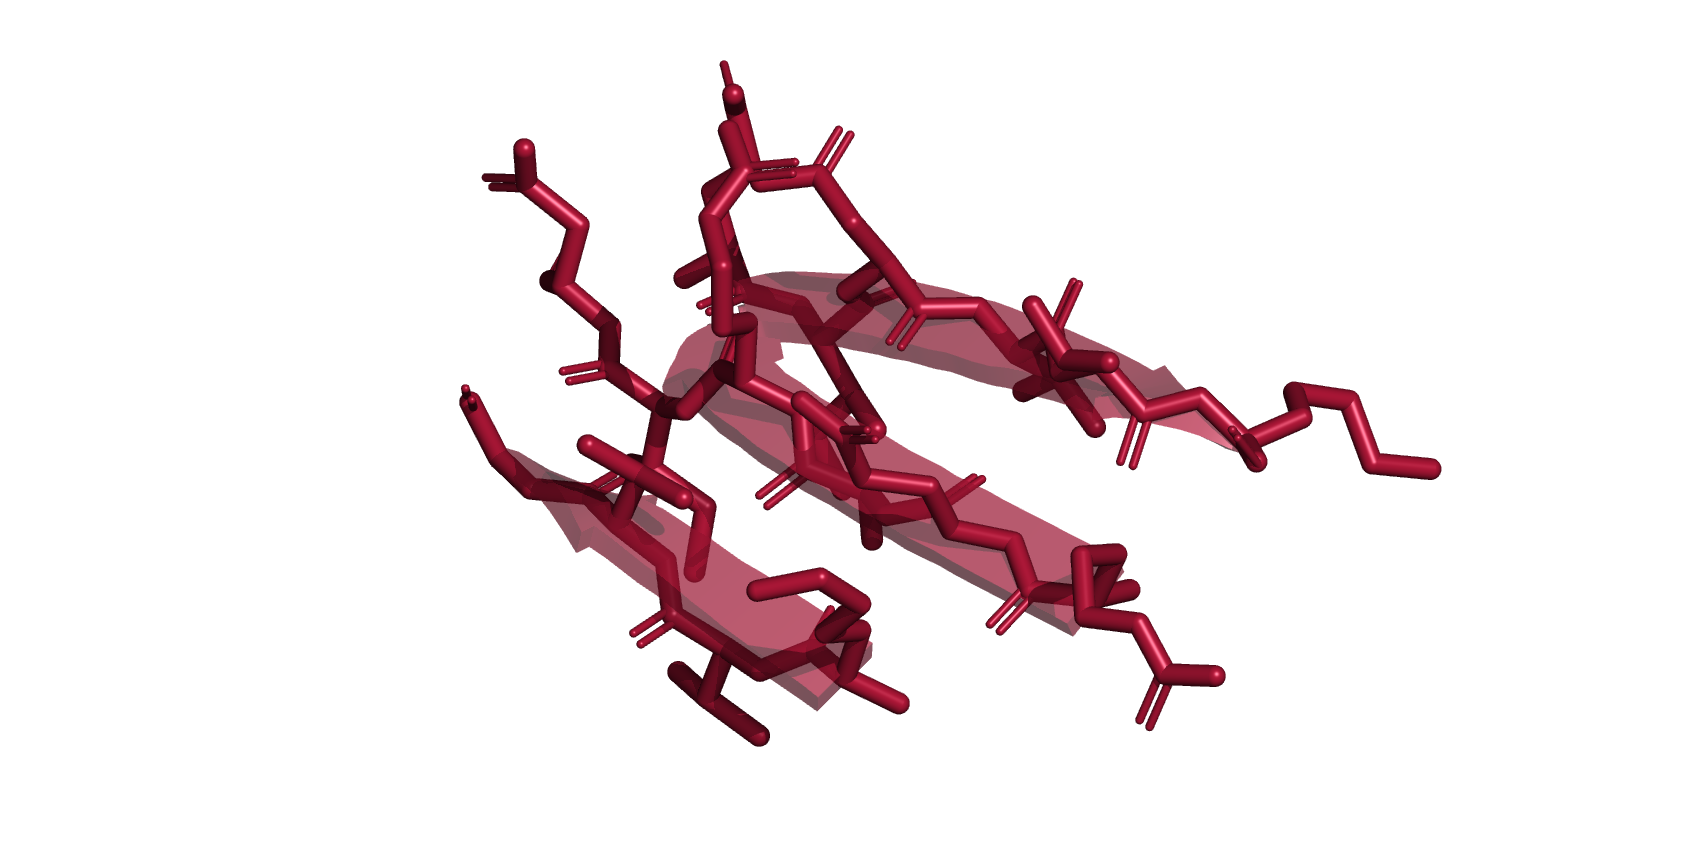
\includegraphics[trim={65mm 3mm 32mm 0},clip, width=0.45\textwidth]{bioinfo/figures/sheet_sticks}}
	\hfil
	\subcaptionbox{Atom-sized spheres\label{subfig:spheres}}{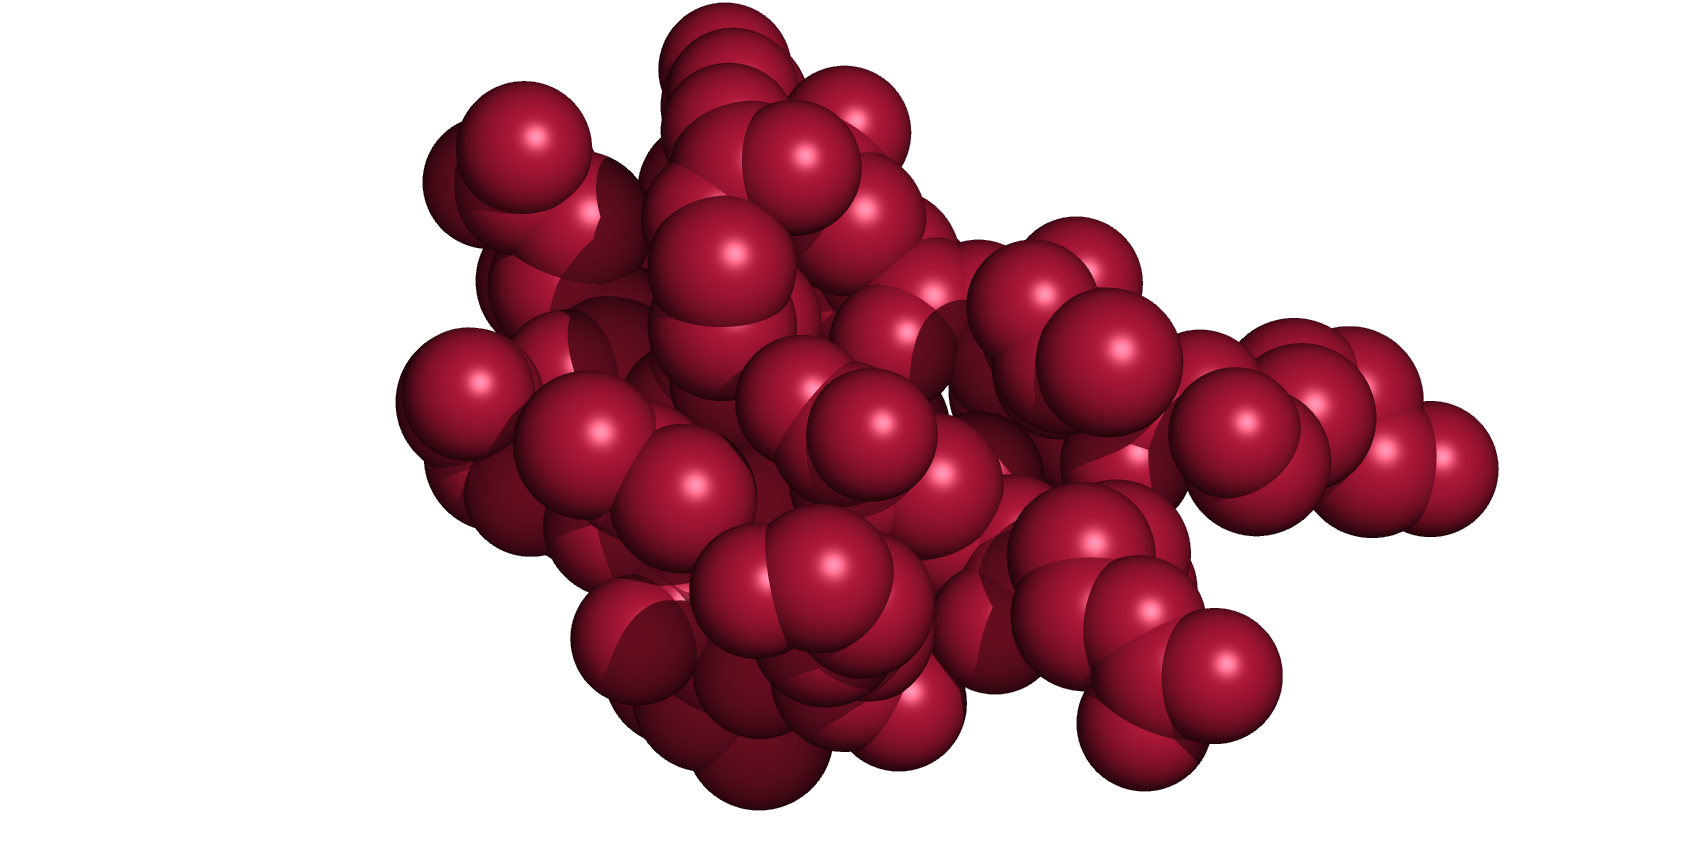
\includegraphics[trim={65mm 3mm 32mm 0},clip, width=0.45\textwidth]{bioinfo/figures/sheet_spheres}}
	\hfil
	\caption{Fragment of a $\beta$-sheet in two representations: cartoon and sticks, and space filling spheres, showing the tightness of the packing.
	They are both seen from the same angle at the same scale.}\label{fig:packing}
\end{figure}


\subsection{Mutual Information}
How can we formalise mathematically correlated mutations?
Mutual Information codifies the information gain that we can obtain for one distribution knowing the other, and considering the relative distributions.
The formula is:

\begin{equation*}
MI\left(i, j\right) = \sum_{x, y}^{q_{max}} f(x_i, y_j) \log \left(\frac{f(x_i, y_j)}{f(x_i)f(y_j)}\right),
\end{equation*}
where $f(x_i, x_j)$ is the joint distribution of amino acids $x_i$ and $y_j$ at positions $i$ and $j$, $f(x_i)$ and $f(y_j)$ are the marginal distributions, and $q_{max}$ is the maximum number of amino acids types in the alignment, including gaps.
Note that if $x$ and $y$ are independent, $f(x_i, y_j) := f(x_i)f(y_j)$, the logarithm vanishes, and thus $M(i, j) = 0$.
If the MSA is of enough quality, the contacts will present high values of $MI$.


\subsection{Direct Coupling Analysis}
Mutual Information has a problem with the transitivity property: consider three residues, A, B, and C; where B is close to both A and C, but A and C are far away.
Mutual Information will likely detect a correlation between A and B, and between B and C; but it will also show a correlation between A and C!

In order to discern true from spurious correlations, we need to fit a statistical model to the whole data at once, in this way, we hope to recover the true (direct) relationships.
This can be accomplished with Direct Coupling Analysis (DCA).
Several variations exist, but they are all based on a Potts model of statistical mechanics.
This is a model where each position (in our case, residue), can take a number of discrete, well-defined, spin states (amino acid types), and the model depends only on the intrinsic properties at each location, and pairwise interactions.

The energy of a sequence of amino acids $\vec{\sigma}$ takes the form:
\begin{equation*}
H(\vec \sigma) = \sum_{\substack{i,j=1\\i \neq j}}^N J_{i, j}(\sigma_i, \sigma_j) + \sum_{i=1}^N h_i(\sigma_i),
\end{equation*}
where $h_i(\sigma_i)$ is the chemical potential of having a given amino acid at position $i$, and $ J_{i, j}(\sigma_i, \sigma_j)$ is the pairwise interaction between residues $i$ and $j$ given their amino acid species.

We can assume the proteins in our MSA were generated by a similar model, so their frequency should follow the Boltzmann distribution:

\begin{equation*}
p(\vec{\sigma} |  h, J) = \frac{1}{Z} e^{-\beta H\left(\vec{\sigma}\right)}
\end{equation*}
$\beta$ is a scaling factor, the inverse of the temperature, and $Z$ is the partition function, a normalisation term to ensure all the probabilities sum up to 1:

\begin{equation*}
Z = \sum_{\vec{\sigma}} e^{-\beta H\left(\vec{\sigma}\right)}
\end{equation*}

Fitting a Potts model means to estimate the values of $J$ and $h$ that best explain the observed distribution of sequences in the MSA.
The problem as such is intractable because computing $Z$ implies a sum over all the possible sequences of length $N$, $21^N$ (the 20 natural amino acids plus the gap state).

There are several strategies that can approximate the partition function, such as plmDCA \citep{plmDCA}, or side-step it all together, like GaussDCA \citep{GaussDCA}.

Once the values of $J$ are obtained, the scores of the contacts can be estimated by taking the Frobenius norm of each of the J matrices.
That is, the square root of the sum of the squares of the couplings between each pair of amino acids:

\begin{equation*}
C(i, j) = \sqrt{\sum_{\sigma_i, \sigma_j=1}^{21} J_{i, j}(\sigma_i, \sigma_j)^2},
\end{equation*}
where $C(i, j)$ is the contact score between residues $i$ and $j$.
This number cannot be readily interpreted as a probability.

This model approximations ignore the possibility of multiple rotamers for a given amino acid \marginpar{The sphericity of the cow}
and consider that any interaction between three or more residues can be decomposed to the sum of each pair.
Finally, DCA attempts to reconstruct the evolutionary couplings, not necessarily the contacts.
\citet{contact_errors} showed that most of the top-scoring pairs indicated by DCA are true contacts, others correspond to contacts between different subunits in a homodimer or pairs of separated residues involved in the function.
The coupling is real, but its nature is different from the model explained at the beginning of this section.

\subsection[Phylogenetic bias]{Phylogenetic bias: the APC correction}
Natural proteins are not randomly drawn from a generative model, like Potts.
Proteins evolve alongside a tree, where a mutation in an organism is likely to be shared among all the descendants.
This appears as a pattern of vertical and horizontal lines on the contact map.

\citet{apc} proposed a simple method to reduce this bias: for each column in the contact map, substract the average of the row times the average of the column, normalised by the total average.

\missingfigure{APC effect}

\subsection{Pattern recognition}
Contacts do not appear at random.
Since the protein is a continuous chain, contacts are rarely isolated, and appear in groups.
Furthermore, since most of the protein is locally organised in secondary structure elements, this gives rise to specific patterns in the contact map.
The statistical methods like DCA and Mutual Information do not consider this, so a refinement step can be done using pattern recognition.
We can train a machine learning algorithm on the outputs of statistical methods and recognise the underlying patterns, which is able to remove much of the spurious contacts, noise, and artefacts in the alignments.

\missingfigure{alpha and beta contacts}

\section{Protein folding}

One of the main goals of protein bioinformatics is predicting the 3D structure of a protein given only its sequence.

\subsection{Physics-based modelling}
Unfolded natural proteins in physiological conditions are known to fold into their native state \citep{fold_graciously}.
In principle, the same procedure can be replicated \emph{in silico} with molecular dynamics, like the work done by \citet{physics_folding}.
This was possible because the domain is very short -- 35 residues --, and fast folding; but in general is not a practical solution, as it requires a lot of computational work.

\subsection{Homology modelling}
Proteins that are close in sequence are close in structure, so if we can find a protein of known structure that has a sequence close to our protein of interest, we can use it as a \emph{template}.
When a good hit is found, this is the most accurate and reliable modelling strategy.

MODELLER \citep{modeller}, for example, uses the templates to infer distance restraints, uses geometrical algorithms to create an initial model, and then relaxes it with a short molecular dynamics run.


\subsection{\emph{Ab-initio} folding}
In the absence of available templates, we can use \emph{ab-initio} or \emph{template-free} methods, in which we try to find the minimum energy of the system, including additional terms derived from predictors.

Rosetta's \citep{Rosetta3} \marginpar{Rosetta} \emph{ab initio} protocol implements a simulated annealing that starts with an extended chain, and randomly replaces fragments with ones derived from the PDB.
Since the fragments are taken from real proteins, the models tend to have good chemical properties, even when completely wrong.
In order to speed up and improve convergence, we can add additional energy terms to the force field, such as contact restraints.

CONFOLD \citep{confold} \marginpar{CONFOLD} is the other protocol used in this thesis.
It is build upon CNS, a NMR reconstruction software, and works by transforming contacts and secondary structure to a large set of distance restraints between atoms.
Then, it runs a geometric solver, followed by a fast relaxation.
This method is much faster than Rosetta, but since it lacks the chemical information of the fragments, it does not work well on regions without contacts.


\subsection{Evaluation}
Once we have a model, how can we compare it with the native structure? How can we measure how accurate it is?

One option is to superimpose model 
\marginpar{Superposition}
in such a way that the metric is optimised.
Given two structures with $L$ residues in common, and being $d_i$ the distance between the $i-$th residues of both structures, we define the distances as:

RMSD, or the Root Mean Squared Deviation:
\begin{equation*}
RMSD = \min \left(\sqrt{\frac{\sum_{i=1}^L d_i^2}{L}}\right),
\end{equation*}

The S-score (Superposition score) is:
\begin{equation*}
S = \max\left[\frac{1}{L} \sum_{i=1}^L \frac{1}{1 + \left(\frac{d_i}{d_0}\right)^2}\right],
\end{equation*}
where $d_0$ is a parameter to be decided, usually $\SI{3}{\angstrom}$.

The TM (Template Modelling score) is the same as S, but $d_0 = 1.24 \sqrt[3]{L - 15} - 1.8$, to keep TM roughly independent of the length.

Both S and TM scores give values between $0$ and $1$.
For TM, values below $0.3$ correspond to random structures, and scores over $0.5$ indicate structures about in the same fold \citep{tmscore05}.

The problem with superposition scores are that are sensitive to conformational changes.
For example, consider a protein composed of two subunits connected by a small, flexible hinge; and a model where each of the subunits is perfect, but the relative orientation is not the same.
The superposition scores would align one of the subunits, with perfect scoring, and give bad values to the other.

A solution is to compare structures locally. 
LDDT (Local Distance Difference Test) \citep{lddt} \marginpar{LDDT}
measures, for every atom, the fraction of preserved  distances, up to a tolerance, within an inclusion radius.
LDDT considers all inter-atomic distances that are within $\SI{0.5}{\angstrom}$, $\SI{1}{\angstrom}$, $\SI{2}{\angstrom}$, and $\SI{4}{\angstrom}$.
The final scores is obtained averaging over all the atoms in the residue and inclusion thresholds.

\citet{cad} proposed a similar method, using surface contacts instead of distances. \marginpar{CAD}
They represent each residue as the Voronoi volume of its atoms.
The surface area for the contact between residues $i$ and $j$ of the model is $S_m(i,j)$, and for the reference -- native structure -- $S_r(i,j)$.
CAD score is proportional to the difference between the two, with some normalisation terms:

\begin{equation*}
CAD_{score} = 1 - \frac{\sum_{i,j} \min\left( \left| \: S_{r}(i, j) - S_{m}(i, j)\right|, S_{r}(i, j)\right)}{\sum_{i,j} S_{r}(i, j)}
\end{equation*}

\subsection[Model Quality Assessment]{Model Quality Assessment, or Estimation of Model Accuracy}
The previous section dealt with the case where we know the native structure, but what can we do when we do not know it?
After all, if we have the experimental data, there is no need for modelling.
The task of predicting the quality of a model is called \emph{Model Quality Assessment} (MQA), or in some modern papers, \emph{Estimation of Model Accuracy} (EMA).
The purpose of MQA is two-fold:

\begin{itemize}
\item \emph{Model selection}, or picking the best model from an ensemble generated by one or different methods.
\item \emph{Model evaluation}, or estimating the overall quality, or how much it can be trusted.
Some applications may require high quality models, while for others, knowing the right fold is sufficient.
\end{itemize}

In principle, \emph{Energy-based MQA?} we could compute the energy of each model, assuming that the lower the energy, the closer we are to our target.
This has two flaws: it does not provide information about \emph{how far} -- since in principle we do not know the energy of the native state -- and it is not a reliable way of comparing models from different methods -- because energy functions are very sensitive to small details.
Consider the case of a perfect model, except for two atoms that are on the same position.
The scores presented on the previous section would all be close to 1, but the energy would be infinite!

We can partially remediate this problem by repacking the models using a common energy function, but this method would still favour models that were optimised with the same energy function we are using.


The alternative solution is to use machine learning and try to predict scores directly.
\marginpar{Unsupervised: clustering}
We can use unsupervised programs, like Pcons \citep{pcons}, that cluster the models, and select the one that is closer to the centre.
The underlying assumption is that, if several independent methods agree, they are probably correct.
If all our models come from a single method, but the set of restraints is good, they will all be similar; but if the restraints are insufficient or contradictory, the models will be diverse.
This is called \emph{consensus methods}.

The alternative is to use supervised machine learning,
\marginpar{Supervised}
describe the model with a set of features, and try to predict in isolation its quality.
The features we can use fall into two categories:

\begin{itemize}
\item Description of physico-chemical properties, such as energy terms and torsion angles.
\item Agreement with predictors, such as secondary structure. A good model should have a good agreement with predictors, but not necessarily perfect.
\end{itemize}

This method is called \emph{single method}, and in this thesis, we have developed supervised methods (Papers \textcolor{Maroon}{I} and \textcolor{Maroon}{IV}).

%\section{Other predictors}
%\todo{TODO}
